
\chapter{Results}

The following results are exploratory in nature, and are 

\section{The self-predicting state}

As a first comparison between the three implmementations, the pre-training towards a self-predicting stat (cf.
\cite{sacramento2018dendritic} Figure S1) was performed with equal parametrizations, as shown in Figure
\ref{fig-self-pred}. For this experiment, no target signal is provided at the output layer, and the network was
stimulated with random inputs.



\begin{figure}[t]
    \centering
    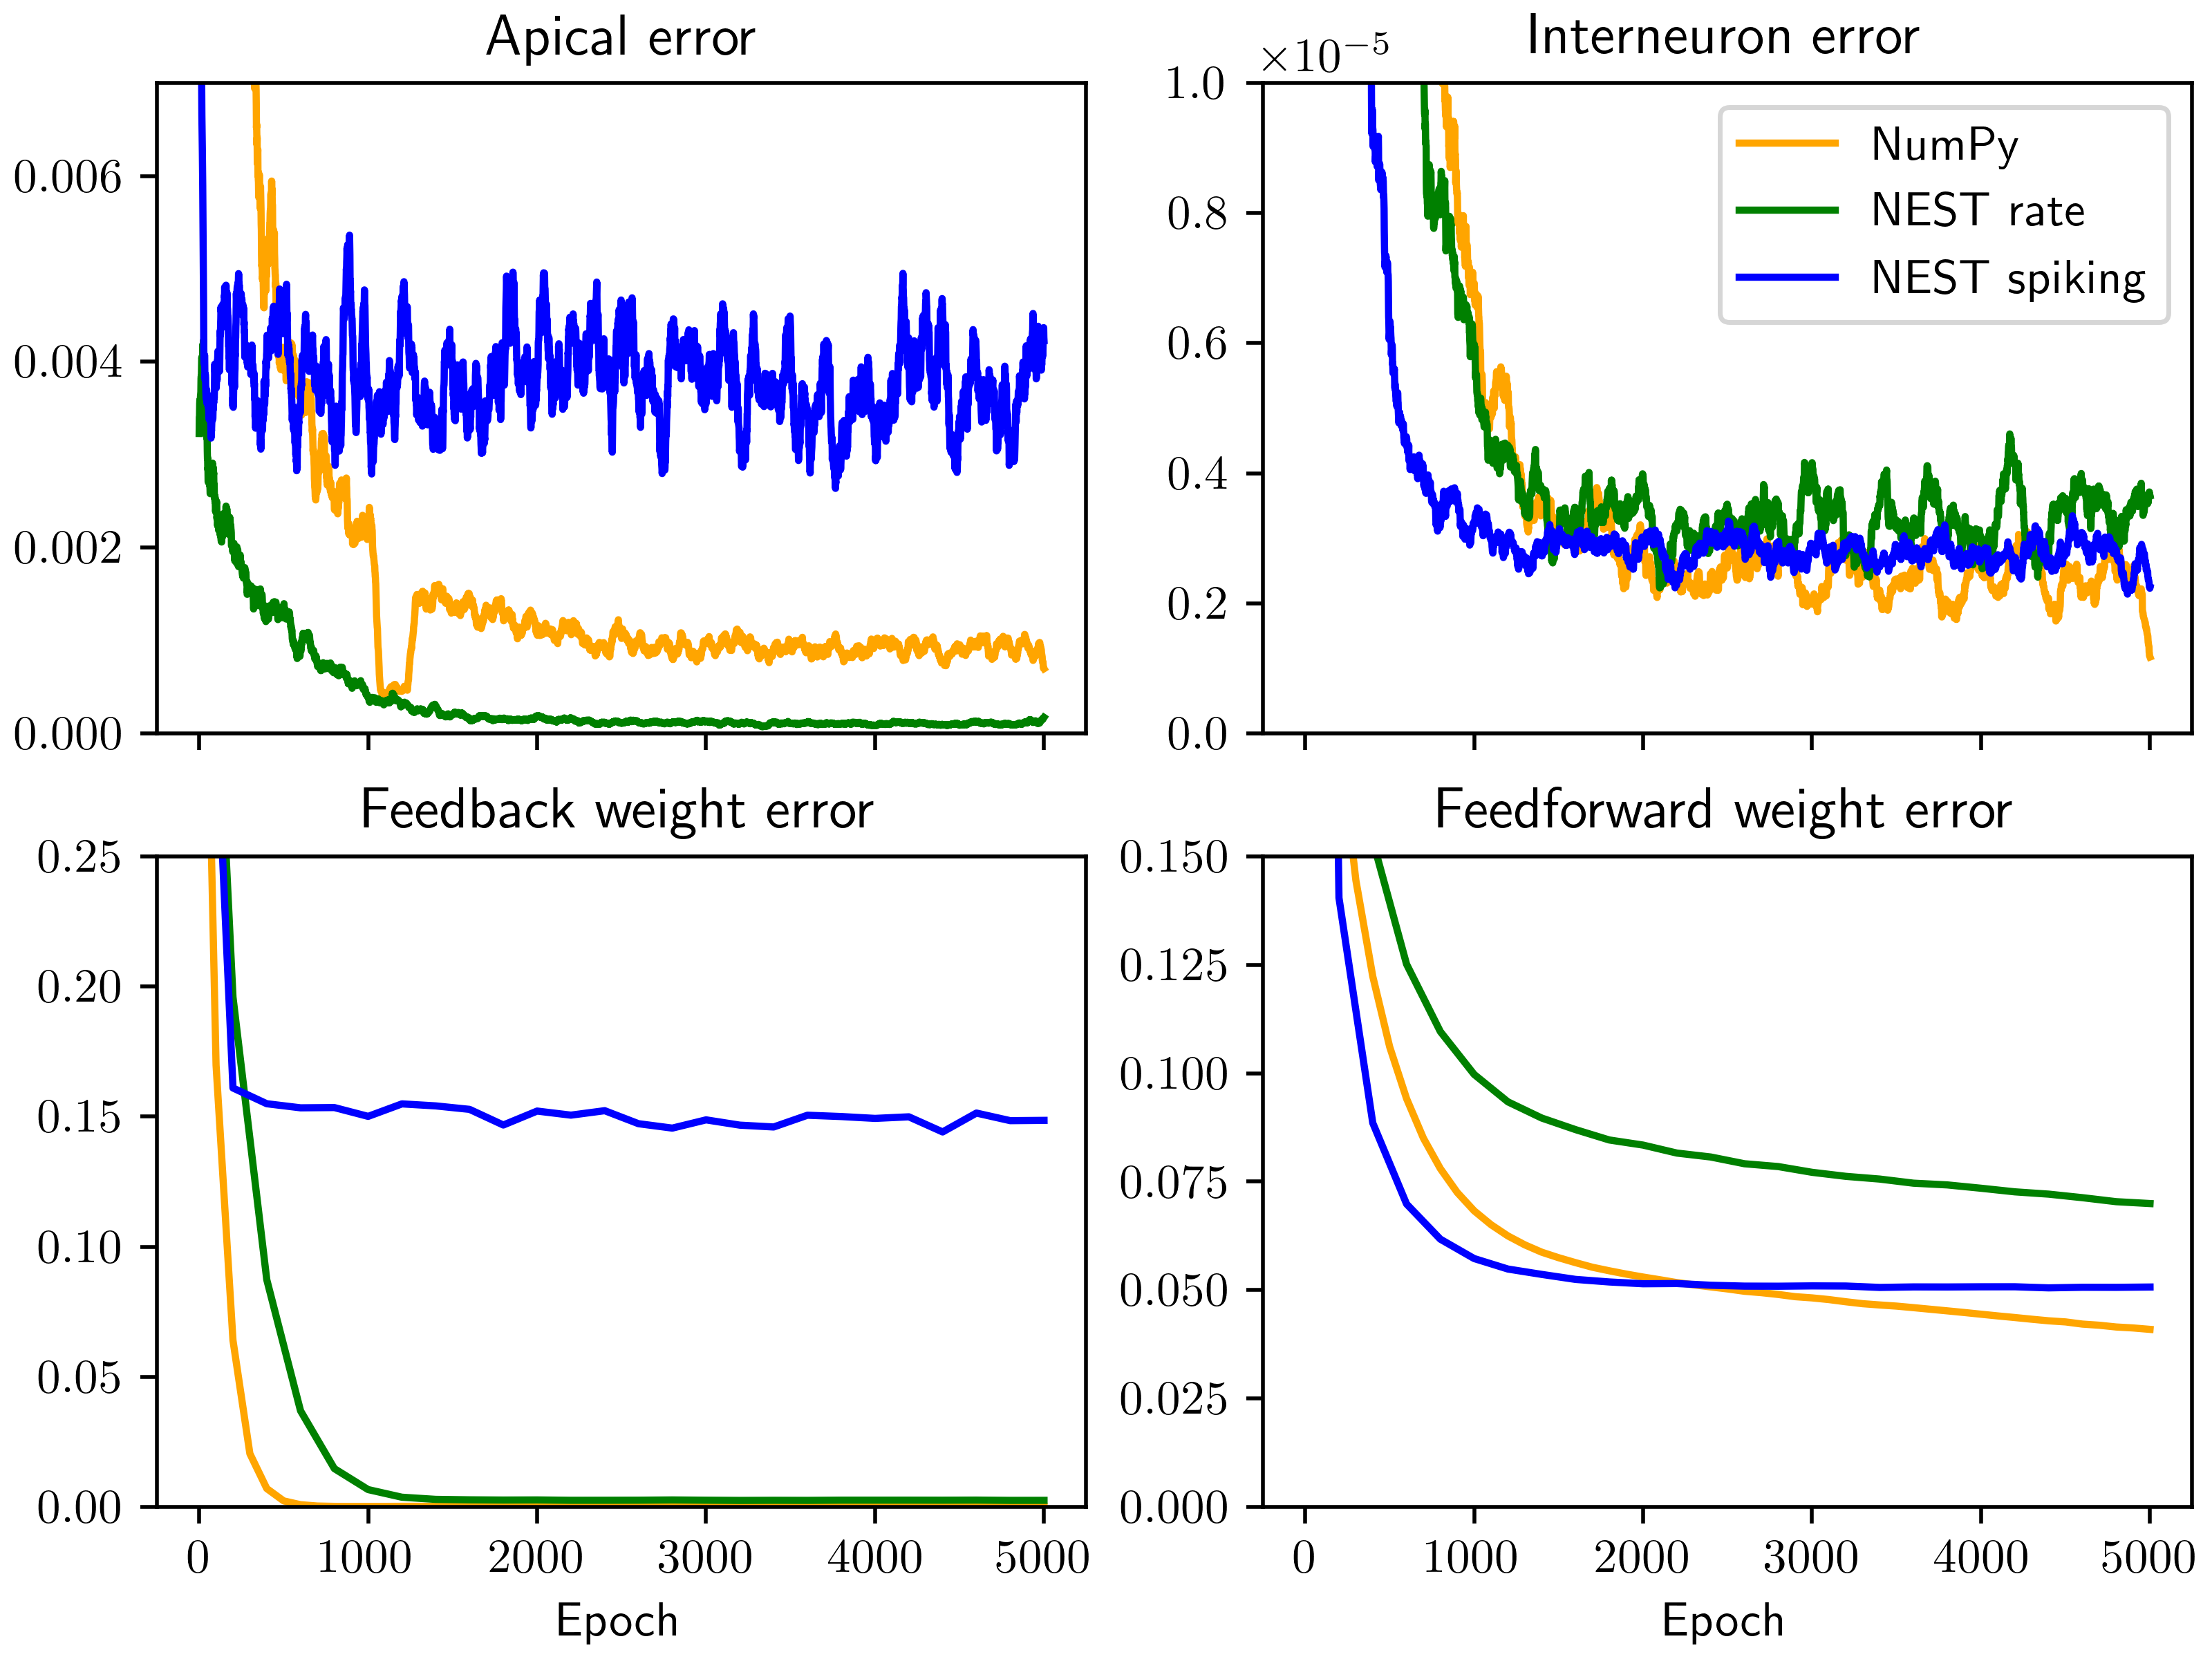
\includegraphics[width=0.9\textwidth]{fig_self_prediction}
    \caption{Different network types learn to predict self-generated activity in superficial layers. All networks were
        initialized with the same random weights for dimensions $[6, 10, 3]$, and stimulated with $5000$ samples of random input for $100ms$ each.
        As described in \cite{sacramento2018dendritic}, during only Pyramidal-Interneuron and Interneuron-Pyramidal
        weights are plastic ($\eta^{pi}=0.05, \eta^{ip}=0.02375, \eta^{up}=\eta^{down}=0$). All variants reach a
        self-predicting state within the first 1000 stimulus presentations and errors remain stable after that point.}
    \label{fig-self-pred}
\end{figure}

All implementations were able to reach comparable values for the four error metrics after roughly the same time. The
exact values that errors converge on differs slightly between implementations, but generally is on the same order of
magnitude and thus does not hinder learning performance greatly (cf. Section \ref{sec-le-tpres}). A notable outlier is
the apical error of pyramidal neuron in the spike-based implementation. This can however be traced back to individual
spikes causing substantial deviations in apical potentials, and can therefore be alleviated by increasing the
\textit{weight\_scale} parameter (results not shown) at the cost of increased training time. Alternatively, increasing
the membrane capacitance of the apical compartment also solves the issue as it smoothes out the effect of individual
spikes. Yet this solution also increases the relaxation period of the entire network, requiring a highly undesirable
increase in $t_{pres}$ for successful learning. Since weight errors converge to similar values as the rate-based
implementations, an increased absolute apical compartment voltage was deemed tolerable.



\section{Apical compartment capacitance}




\section{Presentation times with latent equilibrium}\label{sec-le-tpres}

In order to validate the performance of my implementations, I replicated a parameter study from \cite{Haider2021}[Fig.
    3]. The results for the NEST network using spiking neurons with default parameters \todo{elaborate on this} are
    shown in Figure \ref{fig-bars-le-snest}. A



\begin{figure}[t]
    \centering
    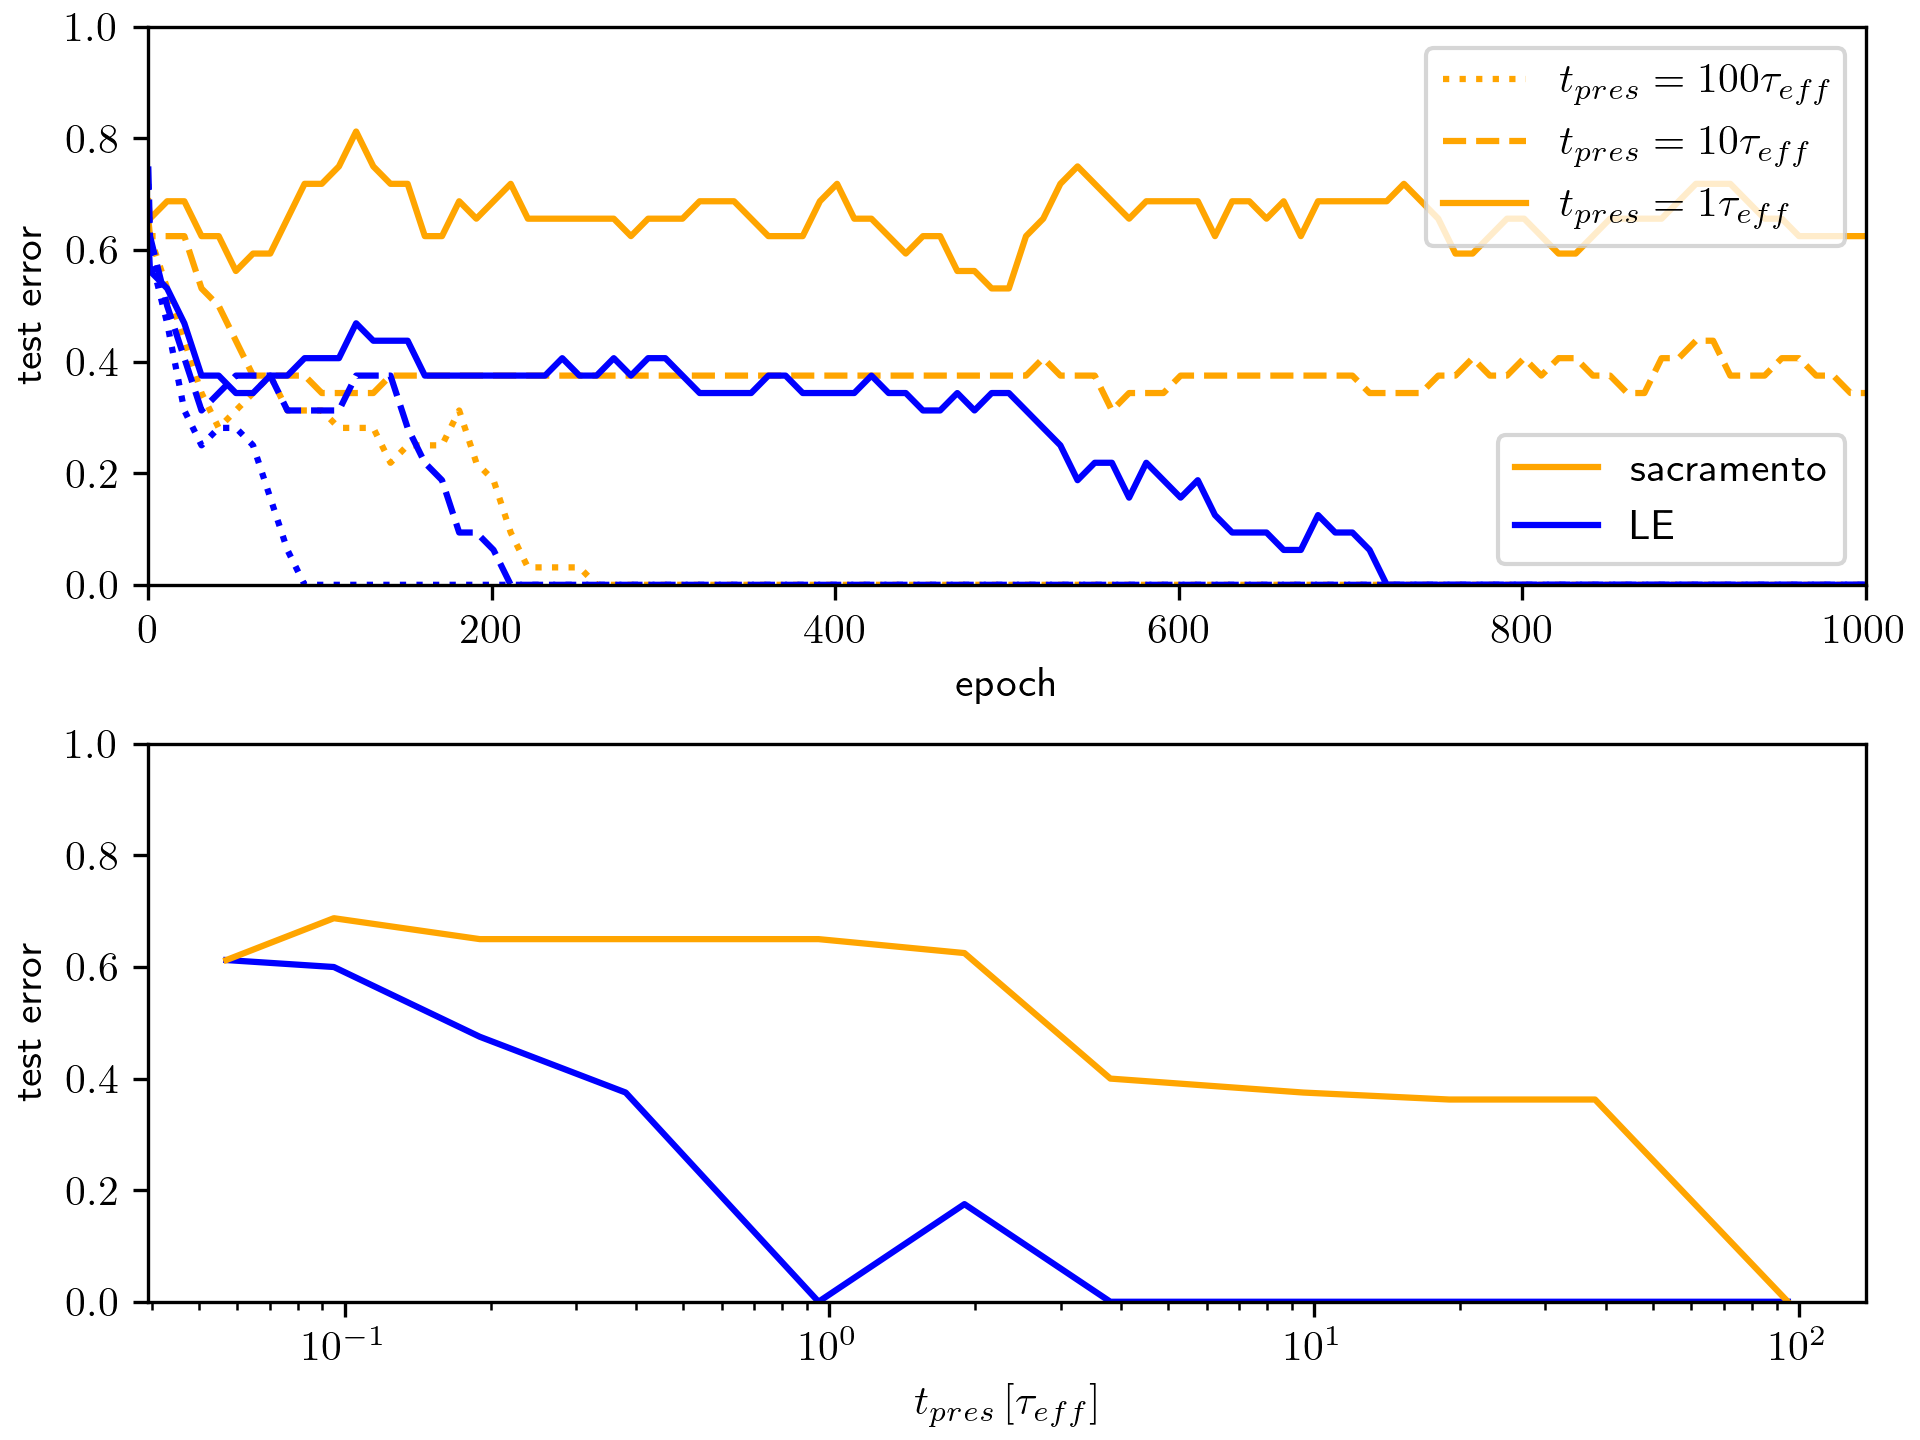
\includegraphics[width=0.9\textwidth]{fig_3_snest}
    \caption{Replication of Figure 3 from \cite{Haider2021} using networks of spiking neurons in the NEST simulator.
        \textbf{A:} Comparison between Original pyramidal microcircuit network by \cite{sacramento2018dendritic} and
        Latent equilibrium variant from \cite{Haider2021}. Shown is the training of a network with 9-30-3 neurons on the
        'Bars' Dataset from \todo{describe it} with three different stimulus presentation times. \textbf{B:} Test
        performance after 1000 Epochs as a function of stimulus presentation time.}
    \label{fig-bars-le-snest}
\end{figure}


\section{Separation of synaptic polarity}
\todo{investigate dales law \citep{Barranca2022}}

A key limitation of the present network model is the requirement that all synapses must be able to assume both positive
and negative polarities. When restricting any synaptic population in the network to just one polarity, the network is
unable to reach the self-predicting state \todo{expand?}. Thus, activity in any neuron must be able to have both
excitatory and inhibitory postsynaptic effects facilitated by appropriate synaptic weights. This requirement is at odds
with biology, which dictates a singular synaptic polarity for all outgoing connections of a neuron, determined by neuron
type and its corresponding neurotransmitter \citeme.


To investigate to what degree the plasticity rule can deal with this constraint, an experiment was conducted: A
 population of pyramidal neurons $A$  was connected to another population $C$ with plastic synapses that were
 constrained to positive weights. In order to facilitate the required depression, $A$ was also connected to a population
 of inhibitory interneurons $B$ through excitatory synapses with random and non-plastic weights. The interneurons in
 turn were connected to $C$ through plastic, inhibitory connections. All incoming synapses at $C$ targeted the same
 dendritic compartment. When inducing a dendritic error in that compartment, all plastic synapses in the network
 collaborated in order to minimize that error. When injecting a positive basal error for example, the inhibitory weights
 ($C \rightarrow B$) decayed, while excitatory synaptic weights ($A \rightarrow B$) increased. Flipping the sign of that
 error injection had the opposite effect on weights, and likewise cancelled the artificial error. This shows that a
 separation of synaptic polarity does not interfere with the principles of the Urbanczik-Senn plasticity when depression
 is facilitated by interneurons.

 \begin{figure}[t]
    \centering
    \begin{minipage}{0.2\textwidth}
        \textbf{a)}\par\medskip
        \centering
        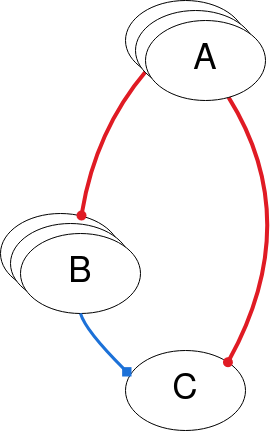
\includegraphics[width=0.9\textwidth]{fig_exc_inh_network}
    \end{minipage}\hfill
    \begin{minipage}{0.7\textwidth}
        \textbf{b)}\par\medskip
        \centering
        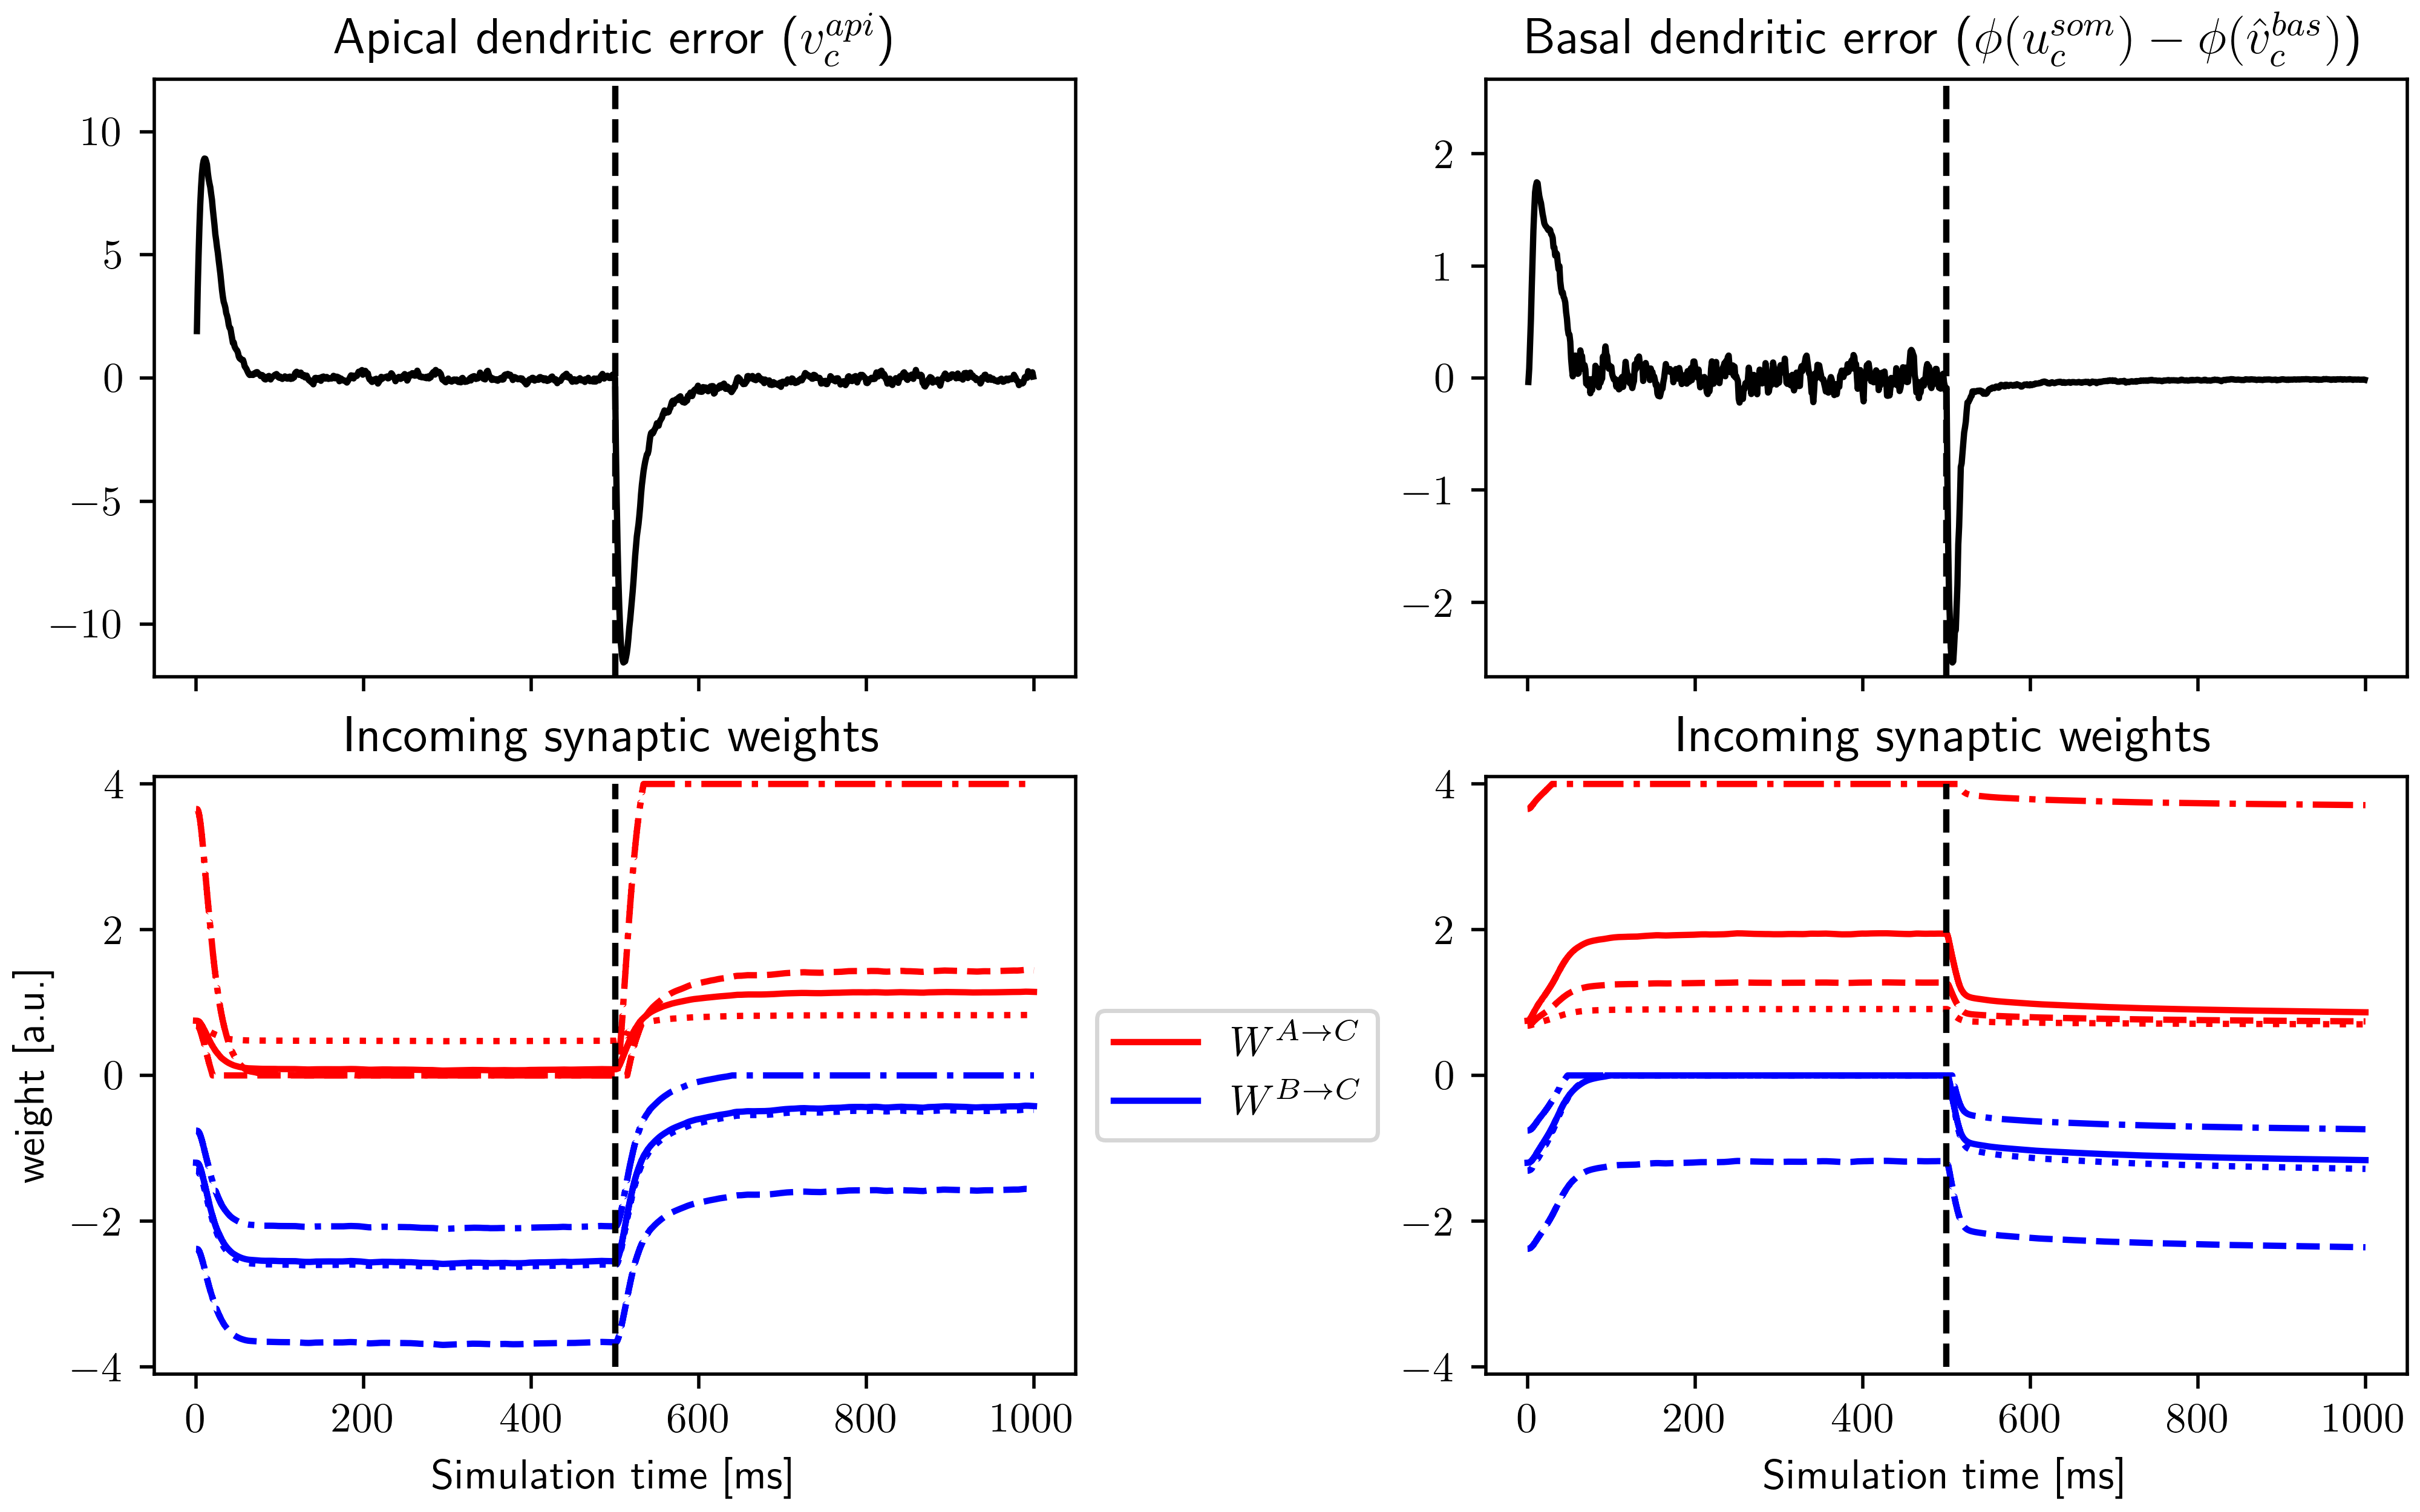
\includegraphics[width=0.9\textwidth]{fig_exc_inh_split}
    \end{minipage}
    \caption{Dendritic error minimization under biological constraints on synaptic polarity and network connectivity.
        \textbf{a)} Network architecture. An excitatory population $A$ connects to a dendrite of Neuron $C$ both
        directly and through inhibitory interneuron population $B$. Only synapses $A\rightarrow C$ and $B \rightarrow C$
        are plastic through dendritic error rules. Populations $A$ and $B$ are fully connected with random weights.
        \textbf{b)} \textit{Left:} All plastic synapses arrive at apical dendrites and evolve according to Equation
        \ref{eq-delta_w_pi}. \textit{Right:} Identical network setup, plasticity for synapses at basal dendrites
        (Equations \ref{eq-delta_w_up}, \ref{eq-delta_w_ip}). \textit{Top:} Dendritic error of a single target neuron.
        Errors of opposite signs are induced at $0$ and $500ms$ (vertical dashed line). \textit{Bottom:} Synaptic
        weights of incoming connections. All initial synaptic weights and input neuron activations were drawn from
        uniform distributions.}
    \label{fig-exc-inh-split}
\end{figure}

Yet, as criticised previously \citep{whittington2019theories}, the one-to-one connections between $A$ and $B$ are
untypical for biological neural networks \citeme. Hence, a second experiment was performed, in which $A$ and $B$ were
fully connected through static synapses with random positive weights. This decrease in specificity of the connections
did not hinder the error-correcting learning, as shown in Figure \ref{fig-exc-inh-split}.

These results are useful, as they enable a biologically plausible way for excitatory long-range pyramidal projections to
connect to pyramidal neurons in another layer (i.e. in a different part of the cortex). The steps required to facilitate
this type of network are rather simple; A pyramidal neuron projection could enter a distant cortical area and spread
spread its axonal tree \phrasing within a layer that contains both pyramidal neuron dendrites and interneurons. If these
interneurons themselves connect to the local pyramidal population, Errors with arbitrary signs and magnitudes in those
dendrites could be effectively minimized by the described connectivity. While error minimization is a funcamental
feature of this network, it does not necessarily imply that synaptic credit assignment is successful aswell. To prove
that this nonspecific connectivity does not hinder learning, it was introduced into the dendritic error network. The
connection between Interneurons and Pyramidal neuron apical dendrites was chosen for the first test, as the employed
plasticity rule had proven most resilient to parameter imperfections previously. A network of rate neurons was
initialized with self-predicting weights as in Section \ref{sec-le-tpres}. The Weights $w^{pi}$ were redrawn and
restricted to postive values, and a secondary inhibitory interneuron population was prepared and fully connected to both
populations as described in Figure \ref{fig-exc-inh-split}. 


\begin{figure}[t]
    \centering
    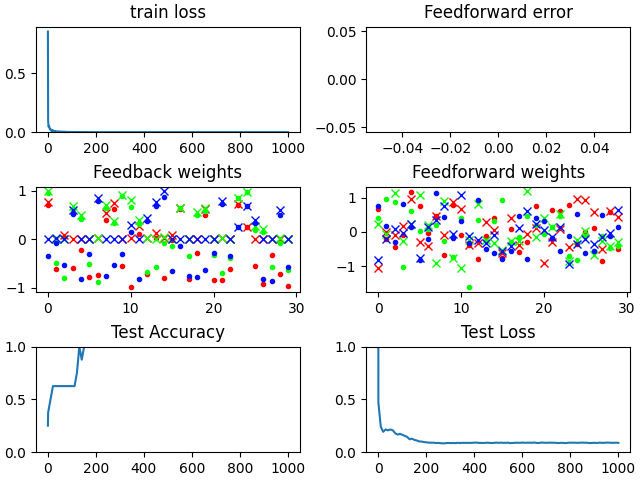
\includegraphics[width=0.8\textwidth]{fig_exc_inh_training}
    \caption{Training progress of a network of rate neurons in NEST, in which hidden layer connections between
    interneurons and pyramidal neurons are unipolar and nonspecific.}
    \label{fig-exc-inh-training}
\end{figure}


\section{In search of plausible spike frequencies}
 \todo{expand}


\section{Resilience to imperfect connectivity}

\begin{figure}[t]
    \centering
    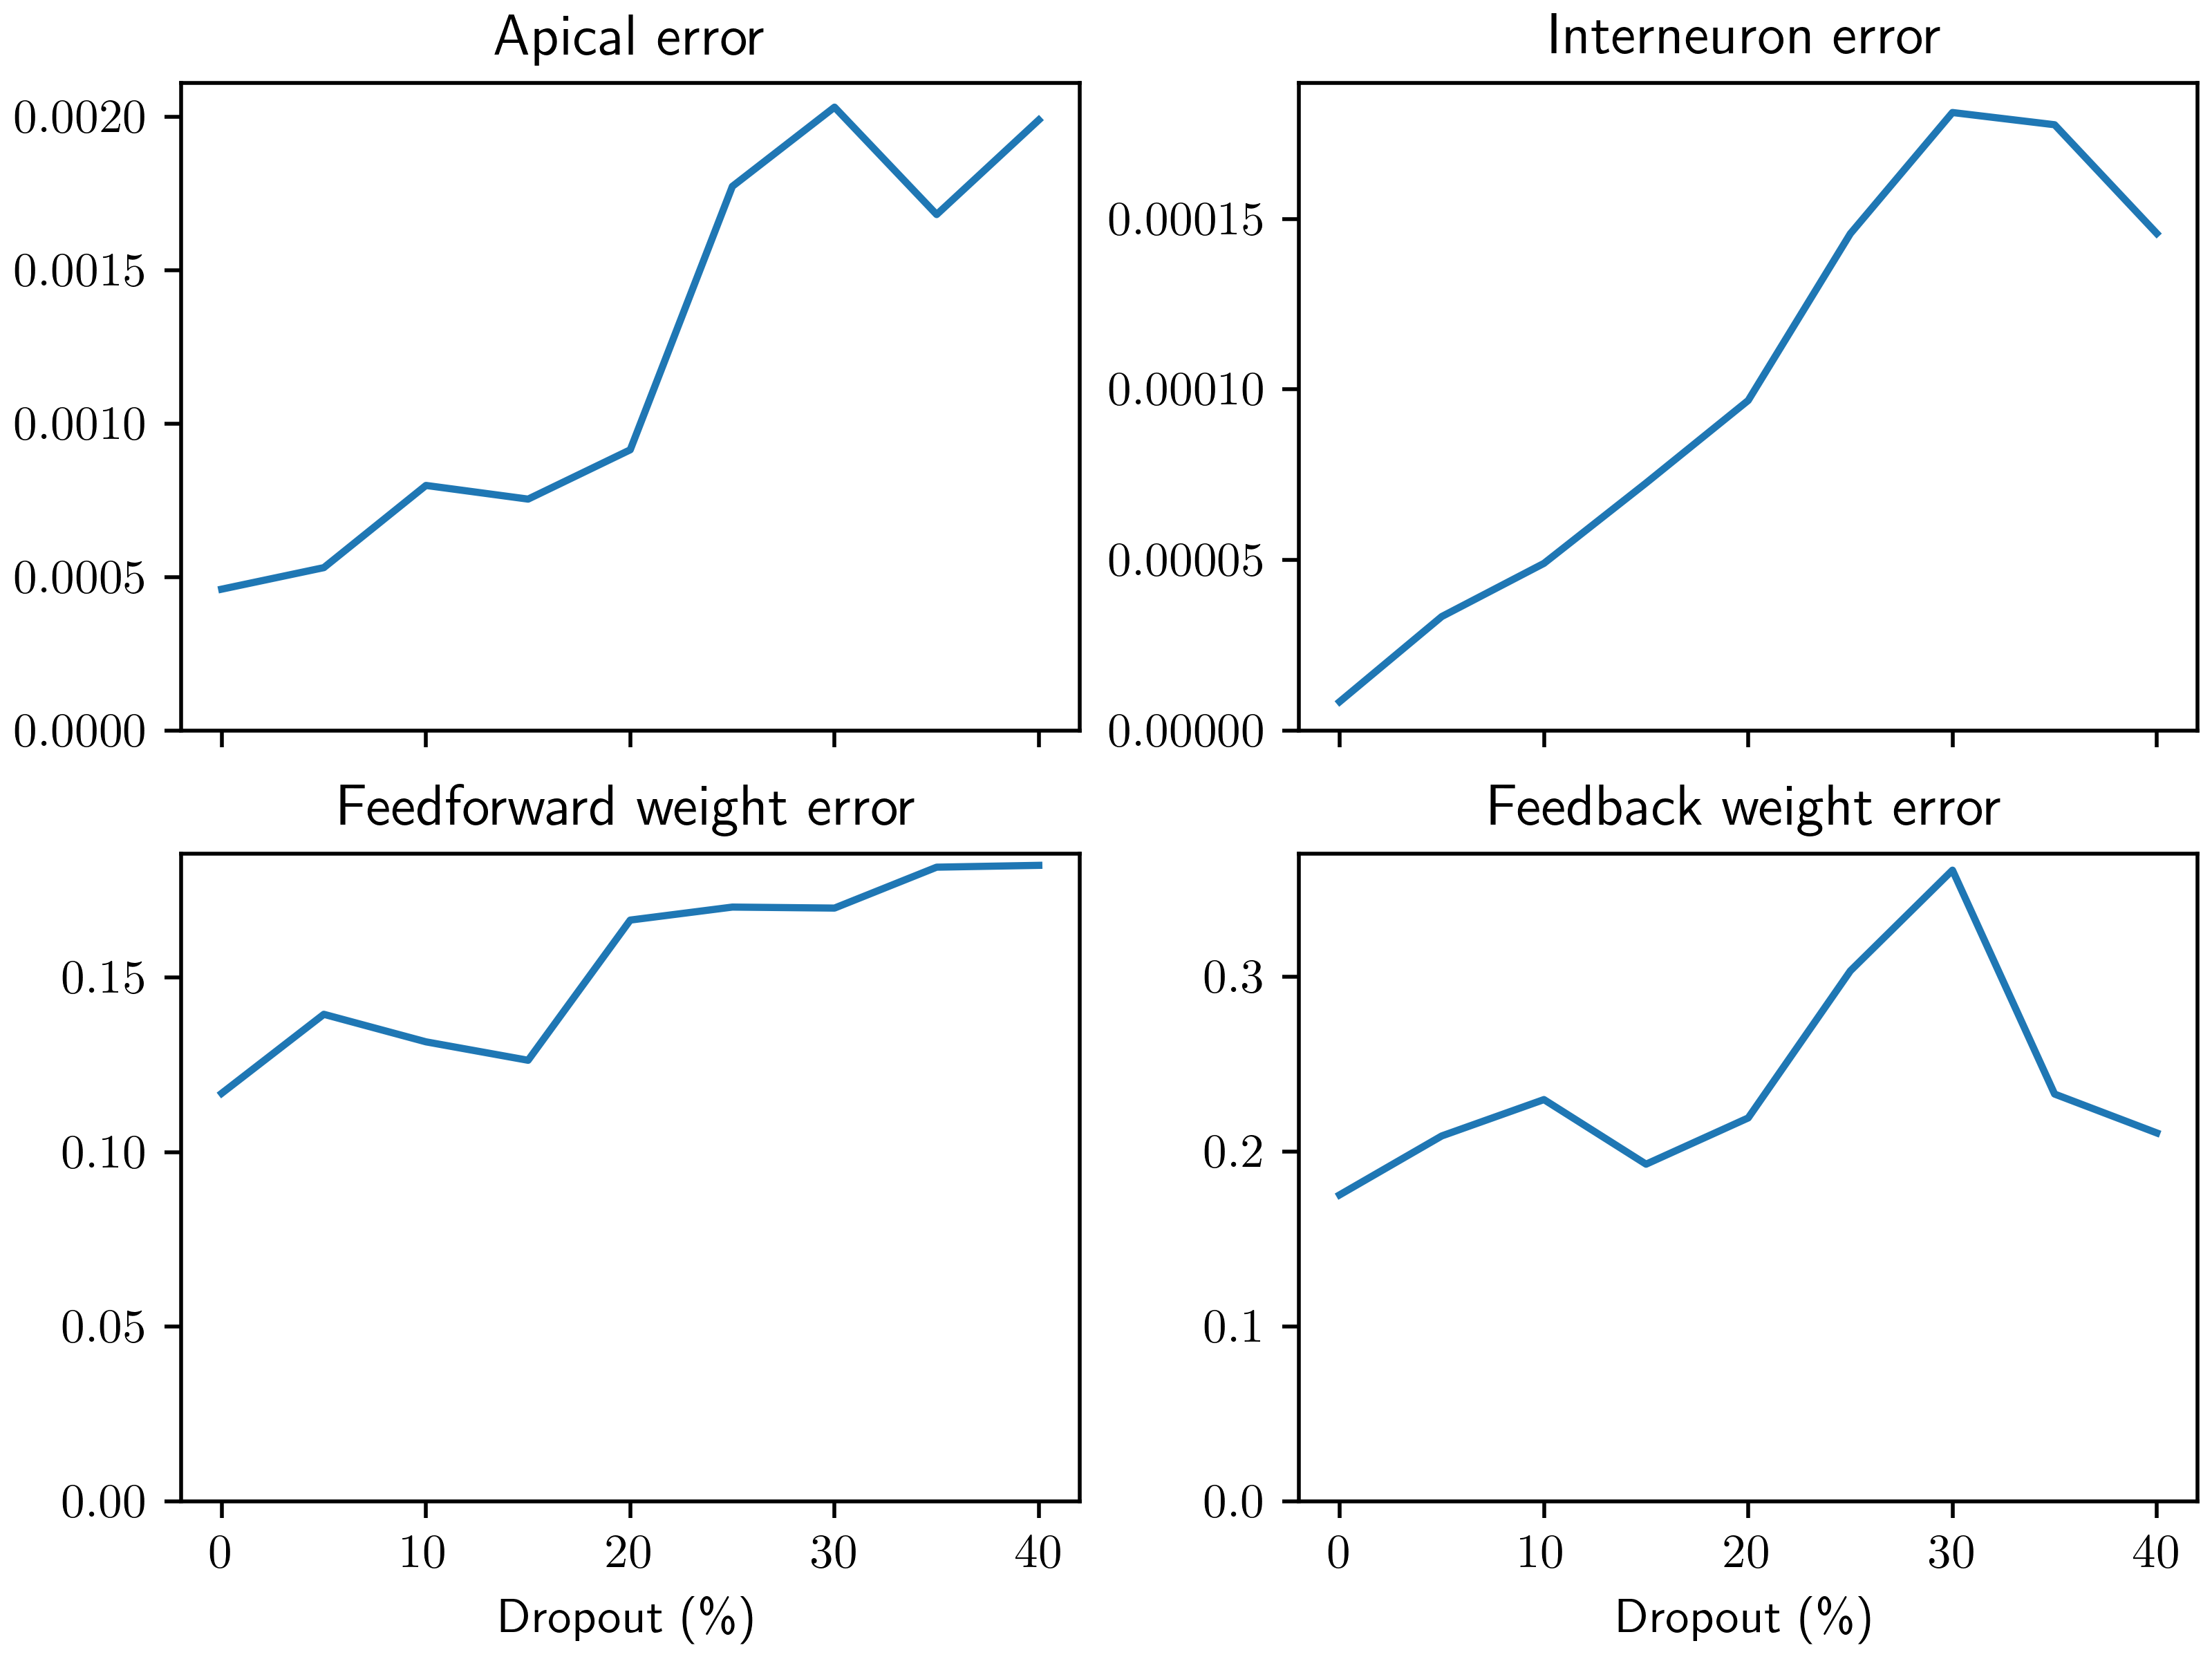
\includegraphics[width=0.9\textwidth]{fig_dropout}
    \caption{Error terms after training a network with dimensions [8, 8, 8] towards the self predicting states, with
    different percentages of synaptic connections randomly removed. To avoid completely separated layers, synapse
    deletion was performed per synaptic population, and the percentage is therefore only an approximation. Even with
    only 60\% of synaptic connections present, the network architecture still achieves competetive values for all four
    error metrics. For the weight errors, which is calculated with mean-squared-error over two matrices, missing
    synapses were set to $0$. This choice was made under the assumption that a missing connection in an ideal
    self-predicting network would be matched by a zero-weight - or likewise absent - synapse. Experiments were performed
    with the rate-based network in NEST, each network was trained fro 2000 epochs of 50ms each.}
    \label{fig-dropout}
\end{figure}


\section{direct feedback connections to interneurons}\label{sec-electric-syns}

\cite{Vaughn2022,Mancilla2007}



\section{Performance of the different implementations}

As stated in \cite{Haider2021}, simulating the present network with many neurons or more than one hidden layer quickly
becomes unfeasible when simulating the full leaky dynamics. To investigate how network size affects simulation time, all
three implementations created for this project were trained on the bars dataset for a single epoch with different
network sizes for a single epoch, in order to assess efficiency.


\begin{figure}[t]
    \centering
    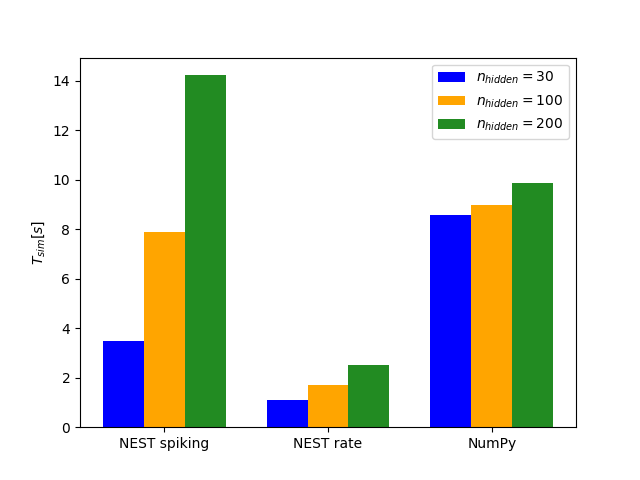
\includegraphics[width=0.8\textwidth]{fig_benchmark}
    \caption{Benchmark of the three different implementations using a network of $[9, n_{hidden}, 3]$ neurons per layer.
        $n_{hidden}=30$ was chosen as a baseline, as it is the default throughout all simulations on the Bars dataset.
        Networks were instantiated with the same synaptic weights and trained for a single epoch of 5 stimulus
        presentations of $100ms$ each. Simulations were performed on an \textit{AMD Ryzen Threadripper 2990WX} using 8
        cores for the NEST simulations at up to $3.0GHz$.}
    \label{fig-benchmark}
\end{figure}

The result of this comparison is shown in Figure \ref{fig-benchmark}. The NumPy network is slow at baseline, which is
likely explained by the fact that it is the only variant which is running on a single thread. This is due to a
limitation of NumPy, and could likely be improved greatly by using batched matrix multiplications, as are provided for
example by \texttt{PyTorch}\footnote{It is also possible, that the network code surrounding the NumPy computations is
less efficient than the one for the NEST network. As this implementation was needed primarily to prove that neuron
dynamics and synaptic updates were ported correctly to NEST, efficiency was a minor concern here and this was not
investigated further.}.  Notably, this variant exhibits very little slowdown in response to an increase in network size.
My assumption is, that the vectorization of synaptic updates on a single thread scales up better than the communication
between threads that is required by most events in the NEST simulations. The NEST implementation using rate neurons
performed best in terms of speed across the board. This result was slightly surprising, as the demand on the
communication interface between threads is very high, since all neurons transmit an event to each of their postsynaptic
targets at every time step.

Finally, the novel spiking variant of this model performed substantially worse than anticipated. Particularly in
comparison to the rate implementation, I initially expected substantial performance improvements. The Difference between
the two was even greater when simulating on an office-grade processor (Benchmark was also run on an \textit{Intel Core
i5-9300H} at $2.40GHz$, results not shown). Three hints about the comparatively poor performance can be deduced: For
one, both the rate and the spiking neuron model employ almost identical neuron models, with minor changes to
parametrization and output generation. Thus, updates to the neuron state are unlikely to be responsible for the worse
performance. Secondly, the number of Events transmitted between neurons is much lower for the SNN compared to

the \textit{relative} performance decrease when increasing the number neurons by the same amout is much greater for the
spiking network. Thus, the most likely cause of slowdown are the updates at the synapses. This is supported by the fact,
that the number of synapses increases much faster for this kind of network than the number of neurons. For the given
network of $n_{x} = 9$ input neurons, $n_y = 3$ output neurons and $n_{h}$ neurons in the hidden layer $l$, the number
of total synapses in the network is given by

\begin{align}
    n_{synapses} & = |w_{l}^{up}| + |w_{l}^{pi}| + |w_{l}^{ip}| + |w_{l}^{down}| + |w_{y}^{up}| \\
                 & = n_h n_x + n_h n_y + n_y n_h  + n_h n_y + n_y  n_h                          \\
                 & = n_h (n_x + n_y^4)
\end{align}

with $|w|$ of a weight matrix $w$ in this case denoting the total number of elements in that matrix \what{Is there a
    more conventional notation?}. Thus, the number of synapses in a network grows much faster than the number of total
    neurons when increasing the size of the hidden layer.

availis given by the stark increase in

\section{Response to unpredicted stimuli}

The activity of many cortical neurons increases when a brain is presented with unpredicted stimuly that regard these
neurons \todo{check out \cite{whittington2019theories} refs 50-54}. This property is prominently replicated by
predictive coding networks, since activation of error nodes is a function of local prediction errors. Prediction errors
in the present model on the other hand are encoded in both positive and negative potentials of apical dendrites. Hence, 
the 

\begin{figure}[t]
    \centering
    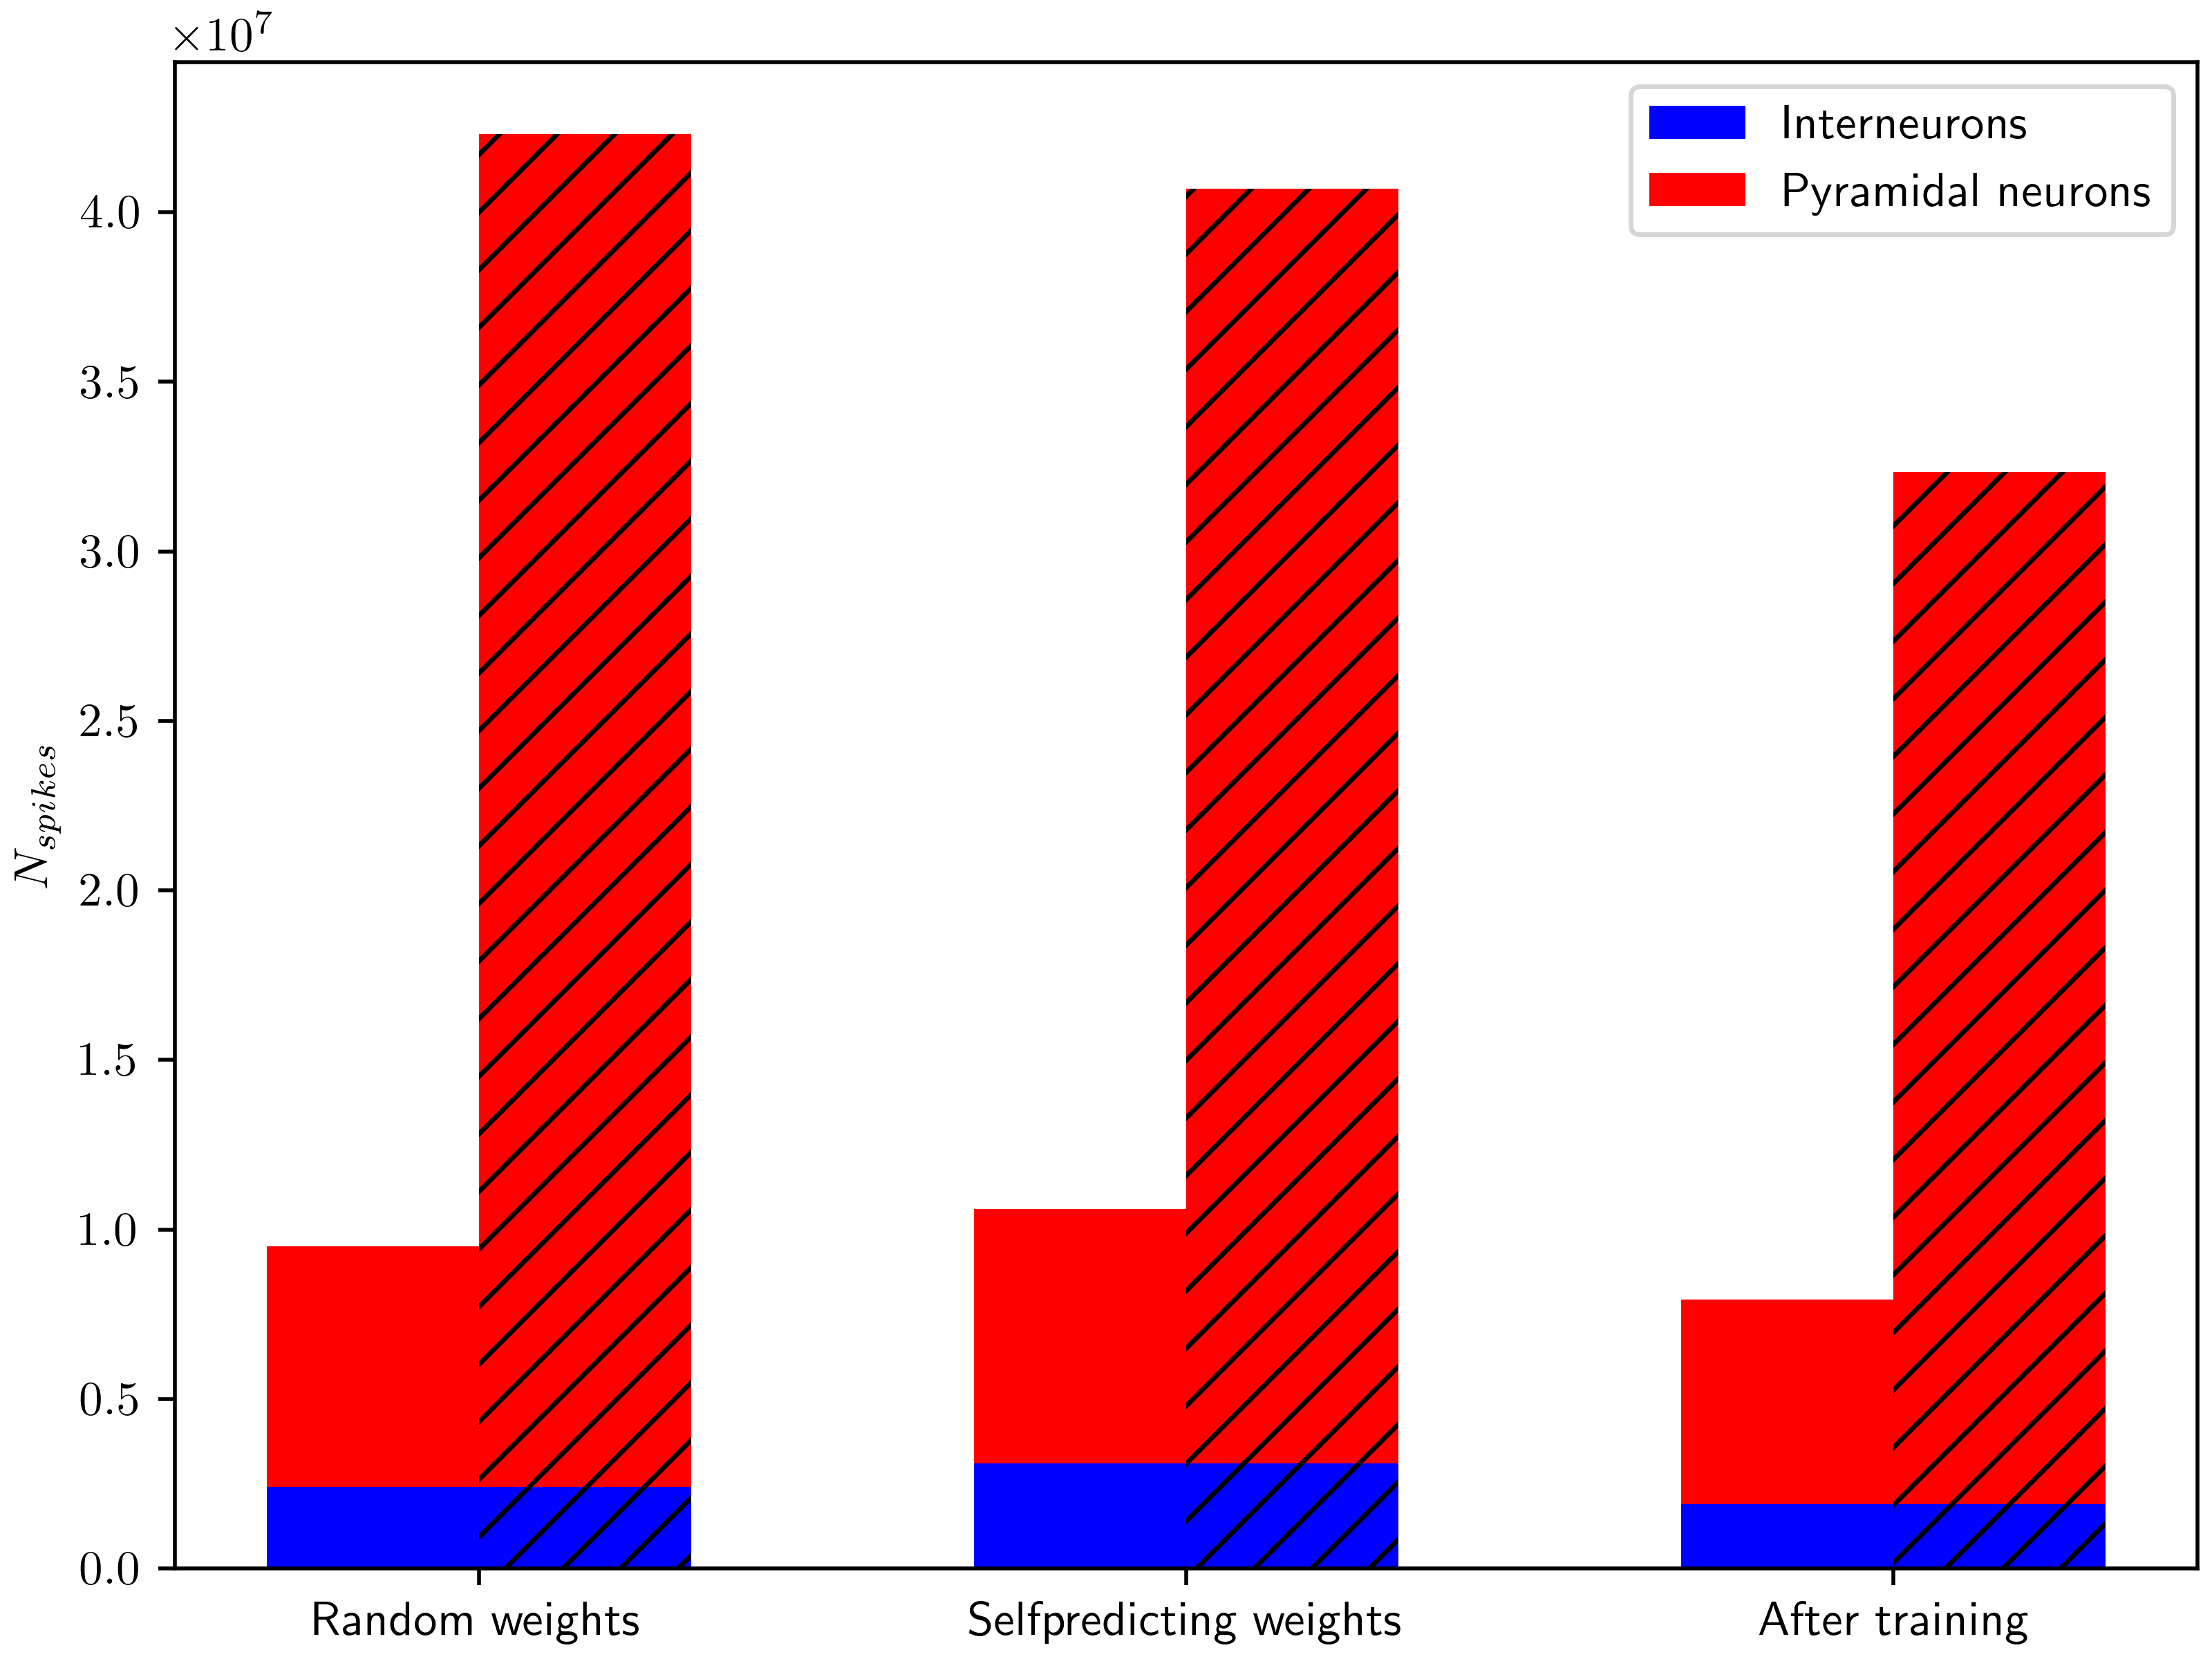
\includegraphics[width=0.9\textwidth]{fig_activity_unpredicted_stimulus}
    \caption{Comparison of network response to stimuli from the Bars dataset.}
    \label{fig-stimulus-response}
\end{figure}




